%       INTRO
%       TRANSFORMÉE MULTI-ÉCHELLE
%       HEURISTIQUES D'ADAPTATION
%       ALGORITHMES
%           CALCULS NIVEAU COURANT
%           CALCUL NIVEAU FIN
%       SOURCES D'ERREURS
%       IMPLÉMENTATIONS
%           MÉTHODES CLASSIQUES 
%           SAMURAI

La multi-résolution adaptative (MRA) est une méthode très efficace pour les problèmes multi-échelles. 
L'objectif est de concentrer les efforts computationnels là où ils sont nécessaires. 
Concrètement cela consiste à augmenter la résolution de la grille de calcul où la solution est complexe et la diminuer où la solution est simple à décrire.
La MRA est donc une méthode de HPC (\textit{high performance computing}) puisqu'elle vise à optimiser l'allocation des ressources de calcul.\par
Cette partie introduit le lecteur à cette méthode en présentant d'abord le concept mathématique de transformée multi-échelle (ou transformée en ondelette)
qui est à la base de la MRA. 
Puis il est expliqué comment la transformée multi-échelle permet d'adapter le maillage pour optimiser la charge computationnelle.
Une fois ces prérequis établis, l'algorithme typique de mise en oeuvre de la multi-résolution adaptative est décrit.
S’ensuit alors naturellement une présentation des différentes implémentations de la MRA, avec une attention particulière sur celle développée au CMAP au travers 
du logiciel Samurai.
Enfin l'impact de la multi-résolution sur la qualité des solutions numériques est abordé. 

\subsubsection{La transformée multi-échelle}
    Cette partie présente la transformée multi-échelle discrète. La transformée multi-échelle continue en simulation numérique,
    c'est bien sûr la version discrète qui est utile.
    Elle se veut avant tout introductive et omets ou simplifie certaines notions; plus de détails sont donnés en \cite{postePoly}.

    \paragraph{Définition mathématique}
        Les explications sont développées en dimensions un à des fins pédagogiques, la plupart des concepts s'entendent naturellement aux dimensions supérieures. 
        De plus, la discrétisation de l'espace se fait selon une grille dyadique, d'autre choix pourraient être fait mais c'est un choix simple, naturel et standard.
        Il faut détailler cette notion.
        \begin{definition}[Grille dyadique]
            Une grille dyadique ou discrétisation dyadique d'un intervalle $I \subset \mathbb R$ est une série de partitions de $I$ indexées 
            par des entiers $j \in J \subset \mathbb N^*$.
            La discrétisation de niveau $j$ correspond à une partitions de $I$ en $2^j$ intervalles (voir fig. \ref{fig:schema_sdyadique}). Ainsi à chaque changement de niveau, du niveau $j$ vers le niveau $j+1$,
            la résolution de la discrétisation est doublée. Les cases de cette partition dyadique sont indexées par deux entiers: $j$ le niveau de résolution de la grille
            et $k$ l'index de la case au sein de ce niveau. En particulier les cases $2k$ et $2k+1$ du niveau $j+1$ correspondent à la case $k$ du niveau $j$.
        \end{definition}
        \begin{figure}[htbp]
    \centering
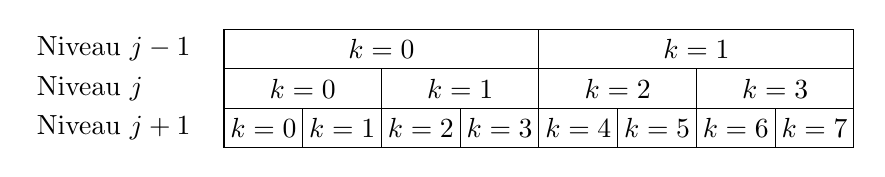
\begin{tikzpicture}


\node[anchor=west] at (-6.5, -.25) {Niveau $j+1$};
\node[anchor=west] at (-6.5, .25) {Niveau $j$};
\node[anchor=west] at (-6.5, .75) {Niveau $j-1$};
% Niveau j-1

\draw (-4,.5) rectangle (0,1);
\draw (0,.5) rectangle (4,1);

    % Niveau j
\draw (-4,0) rectangle (-2,.5);
\draw (-2,0) rectangle (0,.5);
\draw (0,0) rectangle (2,.5);
\draw (2,0) rectangle (4,.5);
%\node at (1,1.75) {$k=2$};

% Niveau j+1

\draw (-4,-.5) rectangle (-3,0);
\draw (-3,-.5) rectangle (-2,0);
\draw (-2,-.5) rectangle (-1,0);
\draw (-1,-.5) rectangle (0,0);
\draw (0,-.5) rectangle (1,0);
\draw (1,-.5) rectangle (2,0);
\draw (2,-.5) rectangle (3,0);
\draw (3,-.5) rectangle (4,0);

% Relations
\node at (-2, .75) {$k=0$};
\node at (+2, .75) {$k=1$};

\node at (-3, .25) {$k=0$};
\node at (-1, .25) {$k=1$};
\node at (+1, .25) {$k=2$};
\node at (+3, .25) {$k=3$};

\node at (-3.5, -.25) {$k=0$};
\node at (-2.5, -.25) {$k=1$};
\node at (-1.5, -.25) {$k=2$};
\node at (-0.5, -.25) {$k=3$};

\node at (+0.5, -.25) {$k=4$};
\node at (+1.5, -.25) {$k=5$};
\node at (+2.5, -.25) {$k=6$};
\node at (+3.5, -.25) {$k=7$};


\end{tikzpicture}
\caption{Exemple de grille dyadique}
\label{fig:schema_sdyadique}
\end{figure}
        Dans ce qui suit il est supposé sans perte de généralité que la discrétisation se fait sur l'intervalle $[0,1]$,
        ainsi le niveau $j$ correspond à des cellules de tailles $1/{2^j}$ et la cellule $k$ du niveau $j$ est centrée en
        $x_k^j = \frac{k+(k+1)}{2} \frac{1}{2^j} = \frac{2k+1}{2^j}.$
        La notion d'ondelette se définit de la manière suivante:
        \begin{definition}[Ondelette]
            Une ondelette est une fonction $\Phi \in L^2(\mathbb R)$ à support compact de moyenne nulle.
            Pour qu'une ondelette soit pertinente dans le cas de la transformée en multi-échelle il est requis
            que la famille $\Bigl(x \mapsto \Phi( 2^j k - x ) \bigr)_{ (j,k)\in \mathbb{Z} \times \mathbb{Z} }$ forme une base de $L^2(\mathbb{R})$.
            En effet la transformée en ondelette sera une projection sur cette base, un peu comme la transformée de Fourrier est une projection sur les 
            fonctions trigonométriques.
        \end{definition}
        Alors la transformée en ondelette discrète peut être définie:
        \begin{definition}[Transformée en ondelette discrète - \textit{Discrete Wavelet Transform, DWT}] Donnée une fonction $f$,
            le coefficient $\gamma_k^j$ de sa DWT sur la cellule $k$ au niveau de résolution $j$ est:
            \begin{align}
                &\gamma_k^j = \frac{1}{N_j} \int_\mathbb{R} \Phi(2^j\cdot k - t)f(t) \text{d} t,\\\notag
                &\text{Où $N_j$ est un coefficient normalisation dépendant du niveau $j$.}
            \end{align}
            Contrairement à une transformée de Fourier, les coefficients ne dépendent pas d'une mais de deux variables. En effet, 
            la transformée en ondelette est plus riche d'informations. Là où la transformée de Fourier ne donne qu'une information 
            sur le contenu fréquentiel d'un signal, la transformée en ondelette donne une information sur le contenu en fréquence \underline{et}
            sur la localisation de ce contenu fréquentiel.
        \end{definition}

    \paragraph{La notion de détails}
        La multi-résolution adaptative se sert de la transformée multi-échelle pour adapter le maillage, c'est à dire compresser l'information (voir \ref{par:adaptation}).
        Cela requiert l'introduction de la notion de détail. Ce concept permet de ne pas utiliser la transformée en ondelette pour quantifier le contenu absolu porté par une échelle particulière,
        mais plutôt à comprendre en quoi ce contenu s'éloigne de ce que les échelles supérieures pourraient laisser supposer, en quoi il est \textit{inattendu}.
        Pour résumer à partir d'un niveau de résolution $j$, on définit un \textbf{prédicteur} polynomial, qui tente d'inférer l'allure de la fonction au niveau $j+1$.
        Puis le \textbf{détail} ne cherche pas naïvement à quantifier et localiser l'information contenue aux échelles du niveau $j+1$ mais plutôt, 
        à quantifier l'écart à la prédiction polynomiale.
        \subparagraph{Le prédicteur}
            Donné un point central $(x_0,y_0)$, et $2s$ voisins $(x_{-s},y_{-s}),(x_{-s+1},y_{-s+1})\dots (x_{s-1},y_{s-1}),(x_s,y_s)$, un prédicteur polynomial 
            ponctuel cherche le polynôme $P$ de degré $2s$ passant par ces $2s+1$ points. Cela permet d'inférer des valeurs pour $y$ en tout point $x$.
            Pour trouver $P(X) = \sum_{k=0}^{2s} a_k X^k$ revient à résoudre le système linéaire:
            \begin{align}
                \forall j \in \{-s,\dots 0 ,\dots,s\}: y_j = \sum_{k=0}^{2s} a_k x_j^k
            \end{align}
            Ce stage se focalise sur les volumes finis, donc ce n'est pas un prédicteur ponctuel, adapté au différences finies (voir \ref{def:vol_finis}), qui est utilisé mais un prédicteur sur la valeur moyenne. 
            Il ne cherche à imposer les valeurs en chaque point mais à fixer la valeurs moyenne sur chaque cellule,
            cela ajoute peu de complexité puisqu'il suffit d'ajouter une intégration lors de l'établissement du système linéaire pour travailler sur les valeurs moyennes.
            Pour l'usage que souhaité ici, il s'agit en d'évaluer la solution sur la cellule $k$ du niveau de résolution $j$ 
            (ce qui correspond à la cellule de centre $x_k^j = (k+1/2) 2^{-j}$) au niveau de résolution supérieure $j+1$,
            il faut donc appliquer le correcteur linéaire centré sur $x_k^j$ en $x_{\pm} = \pm 2^{-(j+1)}$. En pratique cela revient à faire une combinaison linéaire des $2s$ voisins
            qui vient corriger la valeur en $x_k^j$.
            Le prédicteur dépend donc du nombre de voisins pris de part et d'autre, ce nombre noté $s$ et appelé le \textit{stencil} du prédicteur.
            Plus $s$ est grand plus l'opération de prédiction est précise (mais peut éventuellement devenir bruitée\footnote{Ce n'est pas détaillé ici mais le lecteur se réfèrera à la théorie de l'interpollation...})
            et plus elle est coûteuse. Le coût exact n'est pas évident à estimer puisque qu'une combinaison linéaire
            quelques termes se fait en $O(1)$ sur les machines modernes, toutefois quelques subtilités détaillé en \ref{par:adaptation} interviennent.
            Ainsi les valeurs usuelles tu stencil sont généralement $s=1$ ou $s=2$

        \subparagraph{Les détails}
            À présent que le prédicteur à été décrit le concept de détail peut enfin être abordé. On suppose que l'on dispose d'une fonction $\tilde u^j$
            qui soit une approximation de la fonction $u$, au niveau de résolution $j$. Comme vu précédemment, le prédicteur permet d'obtenir une approximation 
            de $u$ au niveau $j+1$ grâce à $\tilde u^j$. Cette prédiction est noté $\hat u^{j+1}$. Les détails à la résolution $j+1$ sont alors définis comme les 
            coefficient de la transformée multi-échelle de la différence entre cette prédiction et la vraie fonction: $u-\hat u^{j+1}$.
            Alors les coefficients de détails n'encode que ce qui n'était pas prédictible par l'interpolateur polynomial. 
            Ce concept de détail est essentiel. 
            En pratique on ne réalise pas l'opération comme expliqué plus haut puisque à prédicteur et ondelette fixés $\Phi$, il existe une \textit{ondelette duale} $\Psi$
            qui permet directement d'obtenir les détails pour la DWT sur $\Phi$ en réalisant une DWT sur $\Psi$ ce qui accélère considérablement les calculs.\par
            Une autre façon de voir la notion de détail est la suivante:
            pour un niveau de résolution $j$ on note $V_j = \text{Vect}\Bigl((Phi_k^j)_k\Bigr)$, c'est à dire l'ensemble de fonction 
            représentables par les ondelettes de niveau $j$.
            Pour les ondelettes classiques\footnote{C'est en tout cas vrai pour les ondelettes de Haar\cite{postePoly}.} la relation suivante est vérifiée
            $V_0 \subset V_1 \subset V_2 \subset \ldots \subset V_N$. Et bien alors l'espace des détails, celui accessible par l'ondelette duale est $Q_{j+1}$
            le supplémentaire de $V_j$ dans $V_{j+1}$, en d'autre terme, il représente toutes les informations, les \textit{détails} contenues dans 
            le niveau d'approximation $V_{j+1}$ qui n'étaient pas prise en compte par $V_j$ (à l'échelle $j$ ce n'était que des détails). 
            Les coefficients de la décomposition par l'ondelette duale sont  Ainsi grâce à l'ondelette duale, 
            il est possible de calculer les coefficients de détails $d_k^j$ qui à chaque montée en résolution n'encode que l'information qui n'était 
            pas contenue dans la décomposition en ondelette au niveau précédent.\par
            Les deux visions ne sont pas rigoureusement les mêmes, la première représente ce qui est réalisé en pratique lors de la MRA, la seconde 
            est la vision standard de la théorie des ondelettes. Toutefois les deux approches ont la même motivation, ne calculer et ne mettre en valeur à chaque
            niveau que ce qui est nouveau, ce qui n'était pas contenu dans les niveaux précédents.
        
        \subparagraph{Intuition sur les détails}
            Lorsque l'on s'intéresse aux coefficients de détails $d_k^j$,
            l'indice $j$ de \textit{dilatation} fixe l'échelle analysée, c'est à dire la longueur d'onde analysée. Par exemple si $j=5$, 
            les coefficients $d^5_k$ donne une information sur l'information portée par les longueurs d'onde de l'ordre de $2^{-5} = 1/32$.
            La variable $k$ précise l'indice de la cellule analysée.
            Par exemple $\Vert d^5_10 \Vert > \Vert d^5_5 \Vert$ signifie que l'information portée par l'échelle $1/32$
            est plus importante au voisinage de la case $10$ qu'au voisinage de la case $5$.
            De même si $\Vert d^j_7 \Vert > \Vert d^{j+1}_{14} \Vert$ cela signifie qu'au voisinage de $x=\frac{7}{2^j}$
            les longueurs d'ondes $\frac{1}{2^j}$ sont plus présentes que les longueurs d'ondes $\frac{1}{2^{j+1}}.$
            Pour se fixer les idées, c'est comme si la transformée de Fourrier n'avait qu'une vision globale du contenu en fréquence, 
            quelle ne voyait que la moyenne sur le domaine de la transformée en ondelette pour chaque longueur d'onde.
            \begin{align}
                \Vert TF\bigl[ f \bigr](\omega = 2^j) \Vert^2 \sim \Vert \sum_{k} d^j_k \Vert^2.
            \end{align}
            \par 
            Grâce à cette notion de détaille la décomposition multi-échelle permet une description de la solution physique où l'apport à la solution de chaque échelle,
            de chaque distance typique est quantifié, les coefficients $d_k^j$ décrivant l'information contenue dans les échelles de l'ordre de $2^{-j}$.
\subsubsection{L'adaptation}\label{par:adaptation}
    \paragraph{La compression par décomposition multi-échelle}
            Pour compresser une fonction (ou une image comme dans le processus \texttt{jpg}), le processus est très simple, il suffit de fixer un seuil de compression $\varepsilon > 0$,
            de calculer les coefficients de détails de la fonction, 
            puis d'omettre (en pratique de retirer de la mémoire) les coefficient dont la norme est inférieure à $\varepsilon$.
            En pratique le coefficient de compression dépend du niveau étudié puisque le volume des cellules mise en jeu chute avec le niveau $j$
            (un détail de $10^{-2}$ à moins d'importance s'il porte sur des cellules de taille $10$ que sur des cellules de taille $10^{-5}$).
            En pratique l'algorithme serait le suivant:
            \begin{enumerate}  
                \item Calculer les coefficients $d_k^j$.
                \item Pour chaque niveau $j$ et chaque coefficient $d_k^j$: Si $\vert d_k^j \vert < \varepsilon_j = 2^{-j}\varepsilon$, alors $d_k^j\leftarrow 0$, les coefficients sont seuillés.
                \item[] Pour reconstruire au niveau de résolution souhaité: utiliser les détails jusqu'au niveau $j$ le plus fin conservé puis utiliser le prédicteur 
                pour interpoler jusqu'au niveau désiré. Le vocabulaire est heureusement choisit, pour compresser on omet les détails négligeables l'on conserve les détails importants.
            \end{enumerate}
    \paragraph{L'adaptation de maillage et l'heuristique d'Harten}
            L'adaptation de maillage, est une variation de la compression par décomposition multi-échelles précédemment décrite. 
            C'est est une opération de compression de solutions physiques \textit{prudente}.
            Les coefficients y sont seuillés de manière moins impitoyable: certains coefficients qui devraient être écartés
            par la compression sont malgré tout préservés. Ce choix se fait sur la base d'intuitions physiques, 
            la plus connue étant \textit{l'heuristique d'Harten}, introduite par Ami Harten \cite{harten1994}, le père de la MRA.
            Elle stipule que même si un coefficient de détail $d_k^j$ devrait être supprimé, si le niveau de détail du niveau supérieur 
            (c'est à dire $d^{j-1}_{\lfloor k/2 \rfloor}$) est particulièrement élevé, par exemple qu'il est par deux fois supérieur au seuil $\varepsilon_{j-1}$,
            alors le coefficient doit être conservé. En d'autre terme, même si la compression considère l'information à l'échelle $j$ négligeable,
            l'intuition physique pose son véto puisque les échelles supérieurs sont de grandes magnitudes et que cela présage que dans 
            les pas de temps a venir les échelles seront nécessaires à la fidèle capture des phénomènes physiques simulés. Par exemple cela peut signifier qu'un front
            d'onde est en train d'arriver dans les zone étudiée, il faut donc que la simulation puisse en capter toute la richesse.
\subsubsection{Algorithmes de simulation numérique}
    \paragraph{Algorithme général}
            L'intégration de la MRA un algorithme de simulation physique se fait de la manière suivante: 
            tous les $n_{MRA}$ pas de temps (éventuellement être à chaque pas de temps), 
            la solution physique est adaptée selon le procédé explicité ci-dessus. Les détails précédemment omis
            devenant nécessaires sont obtenus grâce au prédicteur. Puis la simulation se poursuite à partir de cette grille de calcul adapté.
            L'économie de mémoire se fait puisque tous les détails ne sont pas stockés et l'économie de calculs puisque moins de cellules sont mises en 
            jeu lors du déroulement de l’algorithme de simulation.\par
            Par exemple, en dimension une, si une zone est adapté avec un niveau de détail de niveau 5, la densité de cellule sur lequel il faut réaliser des est de $2^5$
            et la densité mémoire est de $\sum_{j=0}^5 2^j$. Si le niveau le plus fin de la grille est par exemple 9, il y a un gain computationnel théorique de l'ordre de 
            $2^{9-5}=16$ et en terme de mémoire une économie de l'ordre de $\frac{\sum_{j=0}^5}{2^8} > 10$. Ce gain est exponentiel avec la dimension du problème.
    \paragraph{Le cas volumes finis}
            Il faut détailler ce qui signifie \textit{poursuivre la simulation sur la grille de calcul adaptée} dans le cadre des volumes finis.

    \paragraph{Le débat sur la reconstruction}
\subsubsection{Impact sur les solutions}
    \paragraph{}
    \paragraph{}
\subsubsection{Implémentations de la multi-résolution}
    \paragraph{Méthodes usuelles}
    \paragraph{Le logiciel Samurai}